\normaltrue \difficilefalse \tdifficilefalse
\correctiontrue

%\UPSTIidClasse{11} % 11 sup, 12 spé
%\newcommand{\UPSTIidClasse}{12}

\exer{Train simple $\star$ \label{C2:06:35}}
\setcounter{question}{0}\marginnote{\UPSTIcompetence[2]{A3-05}
\UPSTIcompetence[2]{C2-06}}
\index{Compétence C2-06}
%\index{Train d'engrenages simple}
\ifcorrection
\else
\marginnote{\textbf{Pas de corrigé pour cet exercice.}}
\fi

\ifprof
\else
On s'intéresse à la chaîne de transmission de puissance d'un tracteur Fendt. Cette dernière est composée d'un moteur (et d'une pompe) hydraulique (Mh) ainsi que d'un moteur thermique MAN (Mm). 

Le moteur MAN a pour but de fournir de la puissance à la pompe hydraulique et au tracteur (récepteur R). On donne ci-dessous le schéma de la transmission. 
 
\begin{center}
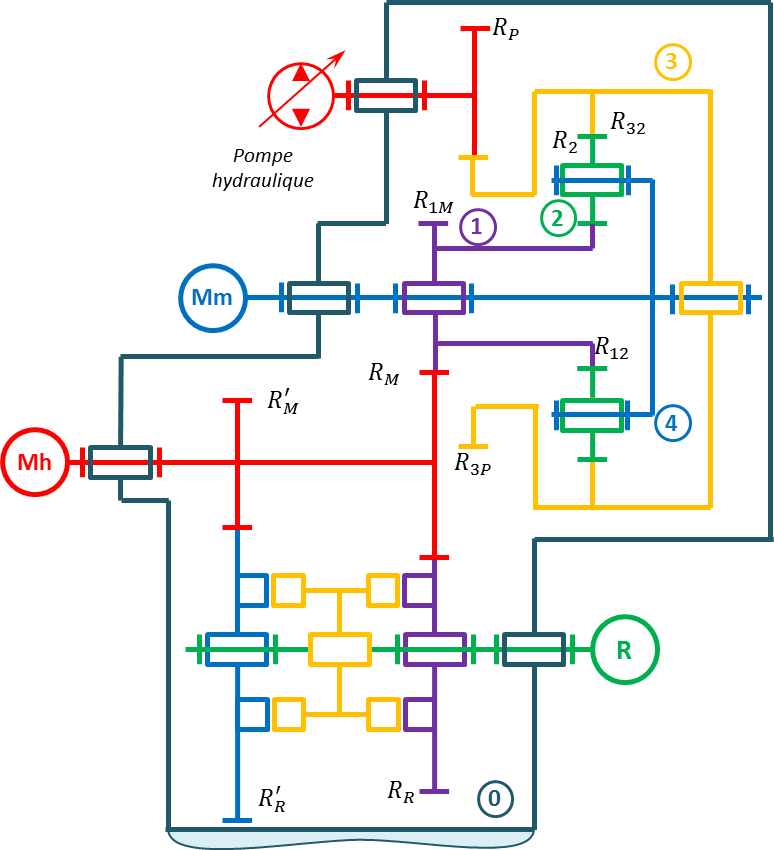
\includegraphics[width=.7\linewidth]{35_01}
\end{center}

Les rayons des pignons sont les suivants : $R_{12}=60$, $R_{1M}=33$, $R_{2}=30$, $R_{32}=120$, $R_{3P}=54$, $R_{M}=54$, $R'_{M}=48$, $R_{R}=42$, $R'_{R}=48$. 

Une étude antérieure a permis d'établir que $\dfrac{\omega(Ph/0)}{\omega(Mh/0)} = \dfrac{2y}{x}$ avec $x\in[0,71;1]$ et $y\in[0;1]$.
%\begin{center}
%\includegraphics[width=\linewidth]{images/fendt_03}
%\end{center}

La fréquence de rotation du moteur Man est de 1900 tr/min.

\fi


\question{Déterminer la relation entre $\omega(1/0)$, $\omega(3/0)$ et $\omega(4/0)$.}
\ifprof
\else
\fi

\question{Montrer que la relation entre la rotation du moteur hydraulique et le moteur Man peut se mettre sous la forme : $\dfrac{\omega(Mh/0)}{\omega(Mm/0)}=-\dfrac{Ax}{BR_py + Cx}$ où on explicitera $A$, $B$ et $C$.}
\ifprof ~\\
On cherche une relation entre $\omega_{\text{Mh}/0}$, $\omega_{\text{Ph}/0}$ et $\omega_{\text{Mm}/0}$ (avec Mm et 4 même classe d'équivalence). Pour cela, on va d'abord rechercher une relation entre $\omega(3/0)$, $\omega(4/0)$ et $\omega(1/0)$.

Bloquons le porte satellite 4, directement lié au moteur Mm. On est alors en présence d'un réducteur simple d'entrée  $\omega(1/4)$ et de sortie $\omega(3/4)$. On a donc : 
$\dfrac{\omega(3/4)}{\omega(1/4)} = -\dfrac{R_{12}}{R_{32}}$. 

En libérant le porte satellite, on a donc :
$ \dfrac{\omega(3/4)}{\omega(1/4)}
= \dfrac{\omega(3/0)-\omega(4/0)}{\omega(1/0)-\omega(4/0)}
= -\dfrac{R_{12}}{R_{32}}
\Leftrightarrow 
R_{32} \omega(3/0) +R_{12}\omega(1/0) = \omega(4/0)\left(R_{12}+R_{32}\right)$

On a donc, $R_{32} \omega(3/0) +R_{12}\omega(1/0) = \omega(\text{Mm}/0)\left(R_{12}+R_{32}\right)$.

Par ailleurs, $\dfrac{\omega(\text{Ph}/0)}{\omega(3/0)} = -\dfrac{R_{3P}}{R_P}$ et 
$\dfrac{\omega(1/0)}{\omega(\text{Mh}/0)} = -\dfrac{R_M}{R_{1M}}$.

On a donc, $ \dfrac{2y}{x} \omega(Mh/0)= -\omega(3/0)\dfrac{R_{3P}}{R_P} \Leftrightarrow  \omega(3/0) = -\dfrac{2y}{x} \dfrac{R_P}{R_{3P}}\omega(Mh/0)$.

En utilisant la relation du train épi :
On a donc, $-R_{32} \dfrac{2y}{x} \dfrac{R_P}{R_{3P}}\omega(Mh/0)  -R_{12} \dfrac{R_M}{R_{1M}} \omega(\text{Mh}/0) = \omega(\text{Mm}/0)\left(R_{12}+R_{32}\right) \Leftrightarrow \left(-R_{32} \dfrac{2y}{x} \dfrac{R_P}{R_{3P}}  -R_{12} \dfrac{R_M}{R_{1M}} \right)\omega(\text{Mh}/0) = \omega(\text{Mm}/0)\left(R_{12}+R_{32}\right)$.


$\dfrac{\omega(Mh/0)}{\omega(Mm/0)}=-\dfrac{R_{12}+R_{32}}{R_{32} \dfrac{2y}{x} \dfrac{R_P}{R_{3P}}  +R_{12} \dfrac{R_M}{R_{1M}}}$

$\dfrac{\omega(Mh/0)}{\omega(Mm/0)}=-\dfrac{\left( R_{12}+R_{32}\right)R_{1M} R_{3P}x }{R_{32} 2y R_PR_{1M} + R_{3P}xR_{12} R_M}$. 
On a donc, $A=\left( R_{12}+R_{32}\right)R_{1M} R_{3P}$, $B=R_{32} 2R_{1M}$ et $C= R_{3P}xR_{12} R_M$. 
\textbf{Attention, plusieurs solutions possibles, si on factorise le numérateur et le dénominateur par l'un ou l'autre des rayons.}
\else
\fi

\ifprof
\else
\begin{flushright}
\footnotesize{Corrigé  voir \ref{C2:06:35}.}
\end{flushright}%
\fi